\section{Voxelización} % (fold)
\label{sec:voxelizacion}
El trazado de conos contra geometria poligonal compleja es costoso. Encontrar los puntos de interseccion entre un cono y un poligono es mas complejo que intersecciones rayo-poligono, ademas de esto un solo cono podria intersectar muchos poligonos.

Para simplificar el trazado de conos se utiliza una discretizacion de la escena en forma de voxeles. Esta representacion puede ser filtrada a niveles mas bajos de detalle. Esto nos permite aproximar el efecto de extender la apertura del cono utilizando cada vez un nivel de detalle mas bajo a traves del recorrido del mismo.

\begin{figure}[H]
	\centering
	\begin{subfigure}[b]{.32\linewidth}
		\centering
		\captionsetup{justification=centering}
		\includegraphics[width=\linewidth]{media/finals/albedo_v256.png}
	\end{subfigure}%
	\hspace{0.01\textwidth}
	\begin{subfigure}[b]{.32\linewidth}
		\centering
		\captionsetup{justification=centering}
		\includegraphics[width=\linewidth]{media/finals/albedo_v128.png}
	\end{subfigure}%
	\hspace{0.01\textwidth}
	\begin{subfigure}[b]{.32\linewidth}
		\centering
		\captionsetup{justification=centering}
		\includegraphics[width=\linewidth]{media/finals/albedo_v64.png}
	\end{subfigure}%
	\caption{Distintos niveles de detalle de una escena voxelizada.}
	\label{fig:voxelization_details}
\end{figure}

Este proceso de voxelizacion para las partes dinamicas de la escena debe ser realizado cada vez que se realiza un cambio sobre alguna superficie que pertenece a algun objeto dinamico en la escena. Por esta razon se requiere un algoritmo de voxelizacion de alto rendimiento para mantener tiempos interactivos.

\subsection{Voxelizacion Conservativa} % (fold)
\label{sub:voxelizacion_conservativa}
Nuestra implementacion realiza voxelizacion conservativa de geometria de alto rendimiento totalmente por \ac{GPU} explotando caracteristicas del pipeline de renderizado de OpenGL. Para esto se implemento el algoritmo de voxelizacion utilizando rasterizacion en hardware explicado en el libro OpenGL Insights por Cyril Crassin y Simon Green en \empty{Octree-Based Sparse
Voxelization Using the GPU
Hardware Rasterizer} \cite{CozziRiccio12}. 

% Esta tecnica utiliza el \emph{geometry shader} y proyeccion ortogonal del triangulo por cada eje para encontrar la maxima area de voxelizacion. La voxelizacion conservativa se logra expandiendo cada vertice del triangulo segun los planos perpendiculares al triangulo por cada par de vertices del mism

Este algoritmo esta basado en el trabajo de Zhang y otros en 2007 \cite{zhang2007conservative} para la voxelization conservativa utilizando la \ac{GPU} y el trabajo de Hasselgren y otros en 2005 \cite{hasselgren2005conservative} sobre rasterizacion conservativa.

Para maximizar el area de rasterizacion la idea es proyectar cada triangulo utilizando proyeccion ortogonal por cada eje direccional. El eje dominante es escogido segun la normal del plano definido por los vertices del triangulo.

\begin{figure}[H]
	\centering
	\captionsetup{justification=centering}
	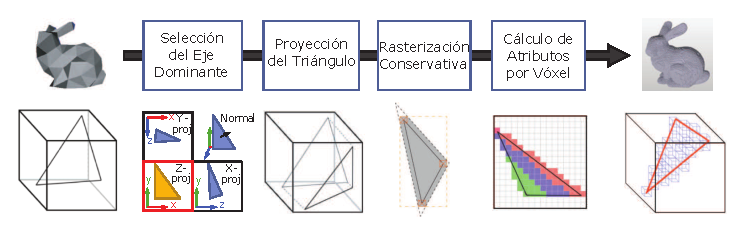
\includegraphics[width=\linewidth]{media/voxelization_pipeline.eps}
	\captaion{Pipeline de voxelizacion utilizado en nuestra implementacion.}
\end{figure}
 
Por cada triangulo proyectado es necesario generar un poligono delimitante un poco mas grande que el triangulo para garantizar la voxelizacion conservativa. Este poligono debe permitir que por cualquier triangulo proyectado tocando un pixel este va obligatoriamente a tocar el centro de este pixel por tanto el pipeline de rasterizacion generara fragmentos para este traingulo. Este poligono se genera expandiendo cada vertice del triangulo hacia afuera utilizando el \emph{geometry shader}. El poligono delimitante no sobreestima la cobertura del triangulo por tanto este no tiene forma de triangulo. Los fragmentos excedentes de este poligono son descartados en el \emph{fragment shader} utilizando un cuboide delimitante.


% subsection voxelizacion_conservativa (end)
% section voxelizacion (end)

\subsection{Voxelización Dinámica} % (fold)
\label{sub:voxelizacion_dinamica}

% subsection voxelizacion_dinamica (end)
